%%%%%%%%%%%%%%%%%%%%%%%%%%%%%%%%%%%%%%%%%%%%%%%%
%% Compile the master file!
%% 		Slides: Antonio Machicao y Priemer
%% 		Course: Wissenschaftliches Arbeiten
%%%%%%%%%%%%%%%%%%%%%%%%%%%%%%%%%%%%%%%%%%%%%%%%


%%%%%%%%%%%%%%%%%%%%%%%%%%%%%%%%%%%%%%%%%%%%%%%%%%%%
%%%             Metadata                         
%%%%%%%%%%%%%%%%%%%%%%%%%%%%%%%%%%%%%%%%%%%%%%%%%%%%  

\title{
	Wissenschaftliches Arbeiten in der Linguistik\\
	(Technische Übung)
}

\subtitle{\LaTeX\ 2: Dokumentstruktur \& Textumgebungen}

\author[aMyP]{
	{\small Antonio Machicao y Priemer}
	\\
	{\footnotesize \url{www.linguistik.hu-berlin.de/staff/amyp}}
	%	\\
	%	{\footnotesize \href{mailto:mapriema@hu-berlin.de}{mapriema@hu-berlin.de}}
}

\institute{Institut für deutsche Sprache und Linguistik}

\date{ }

%\publishers{\textbf{6. linguistischer Methodenworkshop \\ Humboldt-Universität zu Berlin}}

%\hyphenation{nobreak}


%%%%%%%%%%%%%%%%%%%%%%%%%%%%%%%%%%%%%%%%%%%%%%%%%%%%
%%%             Preamble's End                   
%%%%%%%%%%%%%%%%%%%%%%%%%%%%%%%%%%%%%%%%%%%%%%%%%%%%      


%%%%%%%%%%%%%%%%%%%%%%%%%%%%%%%%%%
%%%%%%%%%%%%%%%%%%%%%%%%%%%%%%%%%%
%% Title slide 
\begin{frame}
  \HUtitle
\end{frame}


%% Contents slide
\frame{
\begin{multicols}{2}
	\frametitle{Inhaltsverzeichnis}
%	\tableofcontents[hideallsubsections]
	\tableofcontents
	%[pausesections]
\end{multicols}
	}


%%%%%%%%%%%%%%%%%%%%%%%%%%%%%%%%%%%%
%%%%%%%%%%%%%%%%%%%%%%%%%%%%%%%%%%%%
%% Extra literature

\nocite{Freitag&MyP15a}
\nocite{Knuth1986}
\nocite{Kopka94a}
\nocite{MyP17c}
\nocite{MyP&Kerkhof16a}
	
%%%%%%%%%%%%%%%%%%%%%%%%%%%%%%%%%%%%
%%%%%%%%%%%%%%%%%%%%%%%%%%%%%%%%%%%%


%%%%%%%%%%%%%%%%%%%%%%%%%%%%%%%%%%%%
%%%%%%%%%%%%%%%%%%%%%%%%%%%%%%%%%%%%
%%% Basic literature for these slides

\begin{frame}
\frametitle{Grundlage \& empfohlene Lektüre}

\dots basierend auf \citet{Freitag&MyP15a} und 

auf \citet{MyP&Kerkhof16a}\\
\ras \href{https://www.researchgate.net/publication/279514740_LATEX-Einfuhrung_fur_Linguisten}{LINK}

\end{frame}


%%%%%%%%%%%%%%%%%%%%%%%%%%%%%%%%%%%
%%%%%%%%%%%%%%%%%%%%%%%%%%%%%%%%%%%
\section{Dokumentstruktur}
\frame{
%\frametitle{~}
\begin{multicols}{2}
\tableofcontents[currentsection,hideallsubsections]
\end{multicols}
}
%%%%%%%%%%%%%%%%%%%%%%%%%%%%%%%%%%%

\begin{frame}[fragile]
\frametitle{Dokumentstruktur}

Ein \LaTeX -Dokument besteht (zumindest) aus zwei Teilen: \textbf{Präambel} und \textbf{Body}

\begin{itemize}
\item \textbf{Die Präambel}:

In der Präambel werden alle \textbf{globalen} Eigenschaften des Dokuments definiert. 

	\begin{itemize}
		\item Der \textbf{notwendige Teil} einer Präambel ist der \lstinline|\documentclass{}|-Befehl.
		
		\item[]
		
		\item Optional (entweder in der Präambel oder im Body)
		\begin{itemize}
			\item \textbf{Pakete}, 
			
			\item \textbf{eigene Commands} und 
			
			\item \textbf{Metadaten} 
		\end{itemize}
		
		\item[]
		
		\item Die Präambel \textbf{endet} mit dem \lstinline|\begin{document}|-Befehl. 
	
	\end{itemize}

\end{itemize}
\end{frame}


%%%%%%%%%%%%%%%%%%%%%%%%%%%%%%%%%
\begin{frame}[fragile]
%\frametitle{Dokumentstruktur}

\begin{itemize}
\item \textbf{Der Body}:

Der Body beinhaltet den \textbf{eigentlichen Text} des Dokuments sowie \textbf{lokale Definitionen}.

	\begin{itemize}
	
		\item Er \textbf{beginnt} mit dem \lstinline|\begin{document}|-Befehl  (Ende der Präambel) und
		
		\item[]
		
		\item \textbf{endet} mit \lstinline|\end{document}|. 
		
		\item[]
		
		\item Alles, was diesem \texttt{end}-Befehl folgt, wird von \LaTeX\ nicht interpretiert.
	\end{itemize}
\end{itemize}

\end{frame}


%%%%%%%%%%%%%%%%%%%%%%%%%%%%%%%%%
\begin{frame}[fragile]
%\frametitle{Dokumentstruktur}

%\begin{figure}[b]
	
	\centering
	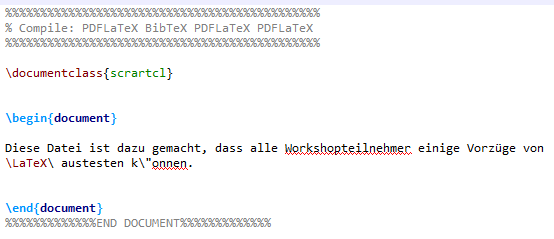
\includegraphics[width=0.9\linewidth]{../../texfiles-beamer/tex-material/WissArb-latex/latexTest1tex}
	
%	\caption{Präambel 1}
%\end{figure}
%
%
%\begin{figure}[b]
	
	\centering
	
\includegraphics[width=0.86\linewidth]{../../texfiles-beamer/tex-material/WissArb-latex/latexTest1pdf}
	
%	\caption{Präambel 2}
%\end{figure}


\end{frame}
	

%%%%%%%%%%%%%%%%%%%%%%%%%%%%%%%%%
\begin{frame}[fragile]
%\frametitle{Dokumentstruktur}

\centering
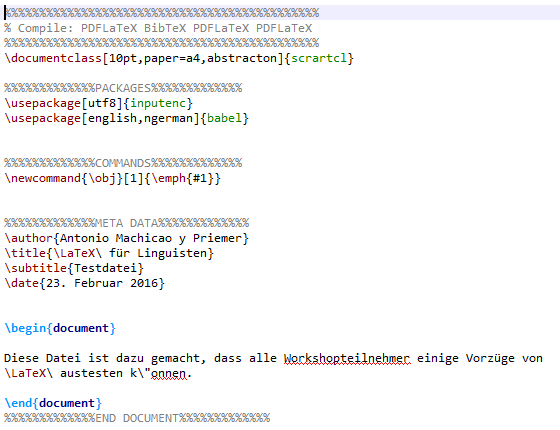
\includegraphics[width=0.9\linewidth]{../../texfiles-beamer/tex-material/WissArb-latex/latexTest2tex}


\end{frame}


%%%%%%%%%%%%%%%%%%%%%%%%%%%%%%%%%
\begin{frame}[fragile]
%\frametitle{Dokumentstruktur}

\centering

\includegraphics[width=0.99\linewidth]{../../texfiles-beamer/tex-material/WissArb-latex/latexTest2pdf}

\end{frame}


%%%%%%%%%%%%%%%%%%%%%%%%%%%%%%%%%%%%
%%%%%%%%%%%%%%%%%%%%%%%%%%%%%%%%%%%%
\subsection{Dokumentklasse}
%\frame{
%	%\frametitle{~}
%	\begin{multicols}{2}
%		\tableofcontents[currentsection,hideallsubsections]
%	\end{multicols}
%}
%%%%%%%%%%%%%%%%%%%%%%%%%%%%%%%%%%%

\begin{frame}[fragile]
\frametitle{Dokumentklasse}

Der \lstinline|documentclass|-Befehl legt die \textbf{Parameter des allgemeinen Dokument-Layouts} fest. Die wichtigsten Klassen sind: 

\begin{itemize}
	\item \texttt{book} für Bücher  
	\item \texttt{report} für längere Schriften mit etlichen Kapiteln, z.\,B. eine Dissertation
	\item \texttt{article} für Artikel, ohne Kapitel nur mit Abschnitten
	\item \texttt{letter} für Briefe
\end{itemize}


\end{frame}


%%%%%%%%%%%%%%%%%%%%%%%%%%%%%%%%%%%%
\begin{frame}[fragile]

Da diese Klassen häufig für \textbf{amerikanische Formate}
spezifiziert sind, gibt es Varianten dieser Klassen, die von
\textbf{\texttt{KOMA-Script}} zur Verfügung gestellt werden (die wir verwenden werden):

\begin{itemize}
	\item \texttt{scrbook} für Bücher  
	\item \texttt{scrreprt} für längere Schriften mit etlichen Kapiteln, z.\,B. eine Dissertation
	\item \texttt{scrartcl} für Artikel, ohne Kapitel nur mit Abschnitten
	\item \texttt{scrlttr2} für Briefe
\end{itemize}

Für Details über das \texttt{KOMA-Script} siehe \citet{Kohm&Co13a} und \url{https://www.komascript.de/}
\end{frame}


%%%%%%%%%%%%%%%%%%%%%%%%%%%%%%%%%
\begin{frame}[fragile]
%\frametitle{Dokumentstruktur}

\centering
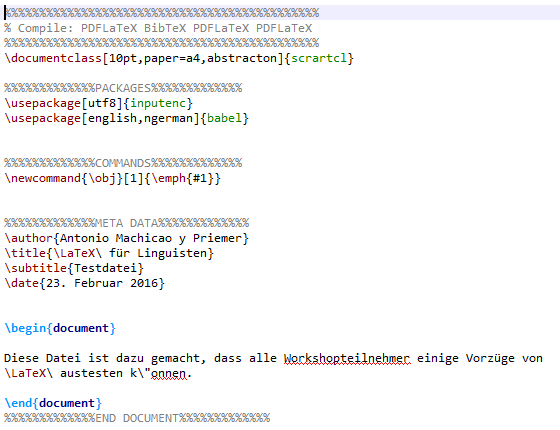
\includegraphics[width=0.9\linewidth]{../../texfiles-beamer/tex-material/WissArb-latex/latexTest2tex}


\end{frame}

%%%%%%%%%%%%%%%%%%%%%%%%%%%%%%%%%%%
\begin{frame}[fragile]
%\frametitle{Dokumentklasse}

Zudem kann man die Optionen dieser Dokumentklassen in dem \ltxterm{documentclass}-Befehl festlegen.

Häufigste Optionen und Minimalbeispiel:

\begin{itemize}
	\item \textbf{Schriftgröße} für die (Default-)Schriftgröße: \ltxterm{10pt}, \texttt{11pt}, \texttt{12pt} \par
	Default $\rightarrow$ \ltxterm{10pt} 
	
	\item \textbf{Papierformat}: \ltxterm{letterpaper}, \ltxterm{a4paper} \par
	Default $\rightarrow$ \ltxterm{letterpaper} \par
\end{itemize}


In den \ltxterm{KOMA-Script}-Klassen sollte man \ltxterm{paper=a4}
oder \ltxterm{paper=letter} statt \ltxterm{a4paper} bzw. \ltxterm{letterpaper} verwenden.

\end{frame}


%%%%%%%%%%%%%%%%%%%%%%%%%%%%%%%%%%%
\begin{frame}[fragile]
\frametitle{Dokumentklasse}

\begin{lstlisting}
\documentclass[10pt,paper=a4]{scrartcl}
\begin{document}
Text Text Text
\end{document}
\end{lstlisting}

\begin{description}
\item[Hinweis:] \ltxterm{TeXstudio} bietet einen Assistenten, der die Präambel für Sie schreibt. Schauen Sie in der Toolbar unter \texttt{Assistenten/Assistent für ein neues Dokument} nach. Dort können Sie alles weitere einstellen.
\end{description}

\end{frame}


%%%%%%%%%%%%%%%%%%%%%%%%%%%%%%%%%%%
%%%%%%%%%%%%%%%%%%%%%%%%%%%%%%%%%%%
\subsection{Pakete einbinden}
%\frame{
%	%\frametitle{~}
%	\begin{multicols}{2}
%		\tableofcontents[currentsection,hideallsubsections]
%	\end{multicols}
%}
%%%%%%%%%%%%%%%%%%%%%%%%%%%%%%%%%%%

\begin{frame}[fragile]
\frametitle{Pakete einbinden}

Die Breite an Funktionen, zu denen man mit \LaTeX\ Zugang hat, ist \textbf{beschränkt}. Um das erwünschte Layout mit den \textbf{Extra-Features} passend zu den eigenen Bedürfnissen zu verwenden, müssen \textbf{zusätzliche Pakete} geladen werden.


Die Pakete müssen in der Präambel mit dem folgenden Befehl geladen werden:
\begin{lstlisting}
\usepackage[parameter1, parameter2]{packagename}
\end{lstlisting}



\end{frame}


%%%%%%%%%%%%%%%%%%%%%%%%%%%%%%%%%%%
\begin{frame}[fragile]


Die Pakete müssen in der Präambel mit dem folgenden Befehl geladen werden:
\begin{lstlisting}
\usepackage[parameter1, parameter2]{packagename}
\end{lstlisting}


\begin{itemize}
	\item Viele der benötigten Pakete sind in der \LaTeX -Distribution (\zB \href{http://miktex.org/}{\ltxterm{MiKTeX}}) \textbf{vorinstalliert}. 
	
	\item (Fast) Alle anderen \textbf{Pakete mit den entsprechenden Benutzerhandbüchern} können kostenfrei aus der Webseite von \textbf{\ltxterm{CTAN}} -- The Comprehensive \TeX\ Archive Network (\href{http://www.ctan.org/}{www.ctan.org}) heruntergeladen werden.
	
	\item Bei Verwendung des \lstinline|usepackage|-Befehls werden die Pakete normalerweise \textbf{automatisch von \ltxterm{MiKTeX} heruntergeladen}.
	
\end{itemize}
\end{frame}


%%%%%%%%%%%%%%%%%%%%%%%%%%%%%%%%%%%
\begin{frame}[fragile]
\frametitle{Pakete einbinden}

Die folgenden Pakete werden häufig benötigt:
\begin{itemize}
	
	\item Kodierung (Input): \ltxterm{inputenc}
	\lstinline|\usepackage[utf8]{inputenc}|
	
	\item Sprachpaket: \ltxterm{babel}
	\lstinline|\usepackage[english,ngerman]{babel}|

	\item Kodierung (Font): \ltxterm{fontenc}
	\lstinline|\usepackage[T1]{fontenc}|
	
	\item Schriftart: \ltxterm{lmodern}
	\lstinline|\usepackage{lmodern}|
\end{itemize}

Die \textbf{Reihenfolge} der Pakete kann von Bedeutung sein! 

\end{frame}


%%%%%%%%%%%%%%%%%%%%%%%%%%%%%%%%%
\begin{frame}[fragile]
%\frametitle{Dokumentstruktur}

\centering
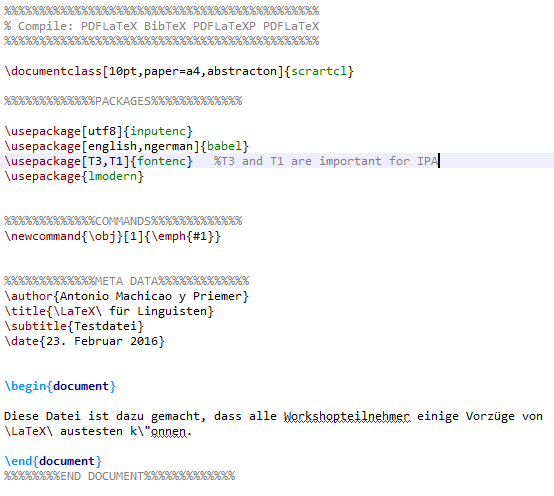
\includegraphics[width=0.75\linewidth]{../../texfiles-beamer/tex-material/WissArb-latex/latexTest3tex}


\end{frame}


%%%%%%%%%%%%%%%%%%%%%%%%%%%%%%%%%%%
%%%%%%%%%%%%%%%%%%%%%%%%%%%%%%%%%%%
\subsection{Metadaten}
%\frame{
%	%\frametitle{~}
%	\begin{multicols}{2}
%		\tableofcontents[currentsection,hideallsubsections]
%	\end{multicols}
%}
%%%%%%%%%%%%%%%%%%%%%%%%%%%%%%%%%%%

\begin{frame}[fragile]
\frametitle{Metadaten}
Zu Beginn des Dokuments können bestimmte \textbf{Metadaten} spezifiziert werden, so zum Beispiel:

\begin{itemize}
\item \lstinline|\author{Vorname1 Nachname1 \and Vorname2 Nachname2}|
\item \lstinline|\title{Dokumenttitel}| 
\item \lstinline|\subtitle{Untertitel}| 
\item \lstinline|\date{23. Februar 2016}| oder \lstinline|\date{\today}| oder \lstinline|\date{}|\par
Default $\rightarrow$ \lstinline|\date{\today}|
\end{itemize}

Mit dem Befehl \lstinline|\maketitle| nach dem Befehl \lstinline|\begin{document}| werden diese Informationen im Dokument wiedergegeben.
\end{frame}


%%%%%%%%%%%%%%%%%%%%%%%%%%%%%%%%%
\begin{frame}[fragile]
%\frametitle{Dokumentstruktur}

\centering
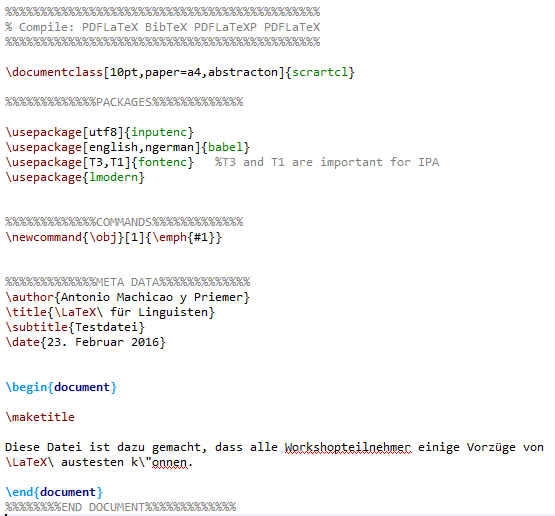
\includegraphics[width=0.72\linewidth]{../../texfiles-beamer/tex-material/WissArb-latex/latexTest4tex}


\end{frame}


%%%%%%%%%%%%%%%%%%%%%%%%%%%%%%%%%
\begin{frame}[fragile]
%\frametitle{Dokumentstruktur}

\centering

\includegraphics[width=0.75\linewidth]{../../texfiles-beamer/tex-material/WissArb-latex/latexTest4pdf}


\end{frame}


%%%%%%%%%%%%%%%%%%%%%%%%%%%%%%%%%%%
\begin{frame}[fragile]

{\small
\begin{lstlisting}
\documentclass[10pt,paper=a4]{scrartcl}

\usepackage[utf8]{inputenc}
\usepackage[english,ngerman]{babel}
\usepackage[T1]{fontenc}
\usepackage{lmodern}

\author{Antonio Machicao y Priemer \and Robyn Kerkhof}
\title{\LaTeX\ für Linguisten}
\subtitle{Eine Einfuehrung}
\date{23. Februar 2016}

\begin{document}

\maketitle

Text Text Text

\end{document}
\end{lstlisting}
}
\end{frame}


%%%%%%%%%%%%%%%%%%%%%%%%%%%%%%%%%%%
%%%%%%%%%%%%%%%%%%%%%%%%%%%%%%%%%%%
\subsection{Textauszeichnung}
%\frame{
%	%\frametitle{~}
%	\begin{multicols}{2}
%		\tableofcontents[currentsection,hideallsubsections]
%	\end{multicols}
%}
%%%%%%%%%%%%%%%%%%%%%%%%%%%%%%%%%%%

\begin{frame}[fragile]
\frametitle{Textauszeichnung}

\LaTeX\ bietet verschiedene Befehle zur Textauszeichnung:

\begin{multicols}{2}

\begin{lstlisting}
\textbf{bold} 
\textit{italics}
\textsl{slanted} 
\emph{emphasized} 
\underline{underline} 
\texttt{typewriter} 
\textsc{small caps} 
ex\textsuperscript{up} 
ex\textsubscript{down} 
\end{lstlisting}

\outputbox{
\textbf{bold}\newline 
\textit{italics}\newline
\textsl{slanted}\newline 
\emph{emphasized}\newline 
\underline{underline}\newline 
\texttt{typewriter}\newline
\textsc{small caps}\newline 
ex\textsuperscript{up} \newline
ex\textsubscript{down} 
}

\end{multicols}
\end{frame}


%%%%%%%%%%%%%%%%%%%%%%%%%%%%%%%%%%%
\begin{frame}[fragile]
%\frametitle{Textauszeichnung}

\LaTeX\ bietet auch die Möglichkeit an, die Schriftgröße zu ändern. Dies ist jedoch in wissenschaftlichen Arbeiten nicht empfehlenswert. Die Schriftgrößenbefehle können entweder als \textbf{Deklarationen} wie auch als \textbf{Umgebungen} angegeben werden.

\begin{multicols}{2}
\begin{lstlisting}
{\tiny tiny} 
{\scriptsize scsize} 
{\footnotesize fnsize} 
{\small small} 
{\normalsize normal} 
{\large large} 
{\Large Large} 
{\LARGE LARGE} 
{\huge huge} 
{\Huge Huge} 
\end{lstlisting} 
\columnbreak{}
\outputbox{
{\tiny{tiny}\newline 
\scriptsize{scsize}\newline
\footnotesize{fnsize}\newline
\small{small}\newline
\normalsize{normal}\newline
\large{large}\newline
\Large{Large}\newline  
\LARGE{LARGE}\newline
\huge{huge}\newline
\Huge{Huge}}
}
\end{multicols}

\end{frame}


%%%%%%%%%%%%%%%%%%%%%%%%%%%%%%%%%%%
%%%%%%%%%%%%%%%%%%%%%%%%%%%%%%%%%%%
\subsection{Gliederung}
%\frame{
%	%\frametitle{~}
%	\begin{multicols}{2}
%		\tableofcontents[currentsection,hideallsubsections]
%	\end{multicols}
%}
%%%%%%%%%%%%%%%%%%%%%%%%%%%%%%%%%%%

\begin{frame}[fragile]
\frametitle{Gliederung}

\textbf{Neue Absätze:} zwei Zweilenumbrüche hintereinander

Weitere Befehle für die lokale \textbf{Strukturierung des Textes} sind:

\begin{itemize}
\item \lstinline|\par| beendet einen Absatz.
\item \lstinline|\newline| und \lstinline|\\| bewirken einen Zeilenumbruch im Outputtext ohne den Absatz zu beenden.
\item \lstinline|\noindent| verhindert die Einrückung nach einem Zeilenumbruch, der jedoch nicht als neuer Absatz markiert werden soll.
\end{itemize}

\end{frame}


%%%%%%%%%%%%%%%%%%%%%%%%%%%%%%%%%%%
\begin{frame}[fragile]
%\frametitle{Gliederung}

\noindent Zudem bietet \LaTeX\ die folgenden \textbf{Gliederungsbefehle}:

\begin{itemize}
\item \lstinline|\part[Kurztitel]{Titel}| 

\item \lstinline|\chapter[Kurztitel]{Titel}| 

(nur in \ltxterm{book} und \ltxterm{report}, bzw.\ in \ltxterm{scrbook} und \ltxterm{scrreprt})

\item \lstinline|\section[Kurztitel]{Titel}|

\item \lstinline|\subsection[Kurztitel]{Titel}| 

\item \lstinline|\subsubsection[Kurztitel]{Titel}| 

\item \lstinline|\paragraph[Kurztitel]{Titel}|

\item \lstinline|\subparagraph[Kurztitel]{Titel}|
\end{itemize}

\noindent In der \textbf{Option \texttt{Kurztitel}} eingegebener Text erscheint im Inhaltsverzeichnis und in den Kopfzeilen.

\vspace{.3cm}

\noindent In der \textbf{Option \texttt{Titel}} eingegebener Text erscheint als Titel im Text.

\end{frame}



%%%%%%%%%%%%%%%%%%%%%%%%%%%%%%%%%%%
%%%%%%%%%%%%%%%%%%%%%%%%%%%%%%%%%%%
\subsection{Inhaltsverzeichnis}
%\frame{
%	%\frametitle{~}
%	\begin{multicols}{2}
%		\tableofcontents[currentsection,hideallsubsections]
%	\end{multicols}
%}
%%%%%%%%%%%%%%%%%%%%%%%%%%%%%%%%%%%

\begin{frame}[fragile]
\frametitle{Inhaltsverzeichnis}

Ein Inhaltsverzeichnis wird durch den folgenden Befehl generiert:
\begin{lstlisting}
\tableofcontents
\end{lstlisting}

\noindent Dieser Befehl muss an der Stelle im Dokument angegeben werden, an der das Inhaltsverzeichnis erscheinen soll. Die Ebenen, die im Inhaltsverzeichnis erscheinen, und die Seitenzahlen werden automatisch von \LaTeX\ aus der Gliederung des Dokuments entnommen (\zB \lstinline|\section[Kurztitel]{Titel}|).

\end{frame}


%%%%%%%%%%%%%%%%%%%%%%%%%%%%%%%%%
\begin{frame}[fragile]
%\frametitle{Dokumentstruktur}

\centering
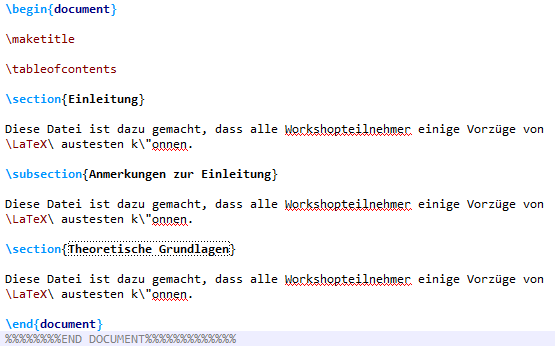
\includegraphics[width=0.84\linewidth]{../../texfiles-beamer/tex-material/WissArb-latex/latexTest5tex}


\end{frame}


%%%%%%%%%%%%%%%%%%%%%%%%%%%%%%%%%
\begin{frame}[fragile]
%\frametitle{Dokumentstruktur}

\centering

\includegraphics[width=0.67\linewidth]{../../texfiles-beamer/tex-material/WissArb-latex/latexTest5pdf}


\end{frame}


%%%%%%%%%%%%%%%%%%%%%%%%%%%%%%%%%%%
%%%%%%%%%%%%%%%%%%%%%%%%%%%%%%%%%%%
\subsection{Fußnoten}
%\frame{
%	%\frametitle{~}
%	\begin{multicols}{2}
%		\tableofcontents[currentsection,hideallsubsections]
%	\end{multicols}
%}
%%%%%%%%%%%%%%%%%%%%%%%%%%%%%%%%%%%

\begin{frame}[fragile]
\frametitle{Fußnoten}

Um eine Fußnote zu generieren, muss nur der folgende Befehl an der Stelle angegeben werden, an der der \textbf{Fußnotenindex} erscheinen soll:

\begin{lstlisting}
\footnote{Inhalt der Fußnote}
\end{lstlisting}

\noindent Beispiel:
\begin{lstlisting}
Hier kommt etwas Text und hier eine Fußnote\footnote{Das 
ist keine Literaturangabe, sondern ein weiterer 
\emph{Kommentar}.} in einer fachlichen Arbeit. 
\end{lstlisting}

\end{frame}


%%%%%%%%%%%%%%%%%%%%%%%%%%%%%%%%%%%
%%%%%%%%%%%%%%%%%%%%%%%%%%%%%%%%%%%
\section{Textumgebungen}
\frame{
	%\frametitle{~}
	\begin{multicols}{2}
		\tableofcontents[currentsection,hideallsubsections]
	\end{multicols}
}

%%%%%%%%%%%%%%%%%%%%%%%%%%%%%%%%%

\begin{frame}[fragile]
\frametitle{Textumgebungen}
\LaTeX\ bietet mehrere Textumgebungen an. Die bekanntesten sind 

\begin{itemize}
	\item Zitate, 
	
	\item unterschiedliche Arten von Listen, 
	
	\item \gqq{wörtliche Wiedergaben} und 
	
	\item Abstracts.
\end{itemize}

\end{frame}


%%%%%%%%%%%%%%%%%%%%%%%%%%%%%%%%%%%
%%%%%%%%%%%%%%%%%%%%%%%%%%%%%%%%%%%
\subsection{Zitate}
%\frame{
%	%\frametitle{~}
%	\begin{multicols}{2}
%		\tableofcontents[currentsection,hideallsubsections]
%	\end{multicols}
%}
%%%%%%%%%%%%%%%%%%%%%%%%%%%%%%%%%%%

\begin{frame}[fragile]
\frametitle{Zitate}
\begin{itemize}
\item Wörtliche Zitate, die länger als zwei Zeilen lang sind, sollen \textbf{vom Fließtext getrennt} werden.

\item \LaTeX\ stellt dafür zwei Umgebungen zur Verfügung: \textbf{\ltxterm{quote}} und \textbf{\ltxterm{quotation}}.

\item Beide Umgebungen sind \textbf{rechts und links eingerückt}.

\item Beide Umgebungen verhalten sich leicht anders je nach Dokumentklasse (\zB Präsentation \vs Artikel).

\item Der Unterschied zwischen den beiden Befehlen betrifft die \textbf{Absatzgrenzen}.

\begin{itemize}
	\item \ltxterm{quote} trennt die Absätze mit vertikalem Abstand, 
	
	\item während \ltxterm{quotation} die erste Zeile jedes Absatzes einrückt.		
\end{itemize}

\item In der \ltxterm{beamer}-Klasse werden Zitate zusätzlich kursiviert.
\end{itemize}
\end{frame}

%%%%%%%%%%%%%%%%%%%%%%%%%%%%%%%%%%%
\begin{frame}[fragile]
\frametitle{Quote-Umgebung}


\begin{lstlisting}
Das ist der Text vor der \texttt{quote}-Umgebung.

\begin{quote}
Die grammatischen Phänomene in einer Sprache zerfallen in zwei 
Teilbereiche: kerngrammatische und randgrammatische Phänomene
(\emph{Ausnahmen}).

\hfill (Nolda et al., 2014)
\end{quote}

Das ist der Text nach der \texttt{quote}-Umgebung.
\end{lstlisting}

\end{frame}


%%%%%%%%%%%%%%%%%%%%%%%%%%%%%%%%%%%
\begin{frame}[fragile]
\frametitle{Quote-Umgebung}

\outputbox{
Das ist der Text vor der \texttt{quote}-Umgebung.

\begin{quote}
Die grammatischen Phänomene in einer Sprache 
zerfallen in zwei Teilbereiche: kerngrammatische und 
randgrammatische Phänomene (\emph{Ausnahmen}).

\hfill (Nolda et al., 2014)
\end{quote}
Das ist der Text nach der \texttt{quote}-Umgebung. 
}

\nocite{Nolda&Co14a}

\end{frame}


%%%%%%%%%%%%%%%%%%%%%%%%%%%%%%%%%%%
\begin{frame}[fragile]
\frametitle{Quotation-Umgebung}


\begin{lstlisting}
Das ist der Text vor der \texttt{quotation}-Umgebung.

\begin{quotation}
Die grammatischen Phänomene in einer Sprache 
zerfallen in zwei Teilbereiche: kerngrammatische und 
randgrammatische Phänomene (\emph{Ausnahmen}).
\end{quotation}
Das ist der Text nach der \texttt{quotation}-Umgebung.
\end{lstlisting}

\outputbox{
Das ist der Text vor der \texttt{quotation}-Umgebung.

\begin{quotation}
Die grammatischen Phänomene in einer Sprache 
zerfallen in zwei Teilbereiche: kerngrammatische und 
randgrammatische Phänomene (\emph{Ausnahmen}).
\end{quotation}
Das ist der Text nach der \texttt{quotation}-Umgebung.
}

\nocite{Nolda&Co14a}

\end{frame}


%%%%%%%%%%%%%%%%%%%%%%%%%%%%%%%%%%%
%%%%%%%%%%%%%%%%%%%%%%%%%%%%%%%%%%%
\subsection{Listenumgebungen}
%\frame{
%	%\frametitle{~}
%	\begin{multicols}{2}
%		\tableofcontents[currentsection,hideallsubsections]
%	\end{multicols}
%}
%%%%%%%%%%%%%%%%%%%%%%%%%%%%%%%%%%%

\begin{frame}[fragile]
\frametitle{Listenumgebungen}

\LaTeX\ hat drei vordefinierte Listenumgebungen:
\begin{itemize}
	\item \ltxterm{itemize},
	\item \ltxterm{enumerate},
	\item \ltxterm{description},
\end{itemize}

\noindent und eine allgemeine Listenumgebung:
\begin{itemize}
	\item \ltxterm{list}.
\end{itemize}

Jeder einzelne Eintrag in Listen beginnt mit \lstinline|\item|.  
\end{frame}

%%%%%%%%%%%%%%%%%%%%%%%%%%%%%%%%%%%
\begin{frame}[fragile]
\frametitle{Itemize}

Die \ltxterm{itemize}-Umgebung wird für ungeordnete Listen verwendet. 

\begin{multicols}{2}
\begin{lstlisting}
\begin{itemize}
  \item erster Punkt
  \item zweiter Punkt

  \begin{itemize}
    \item Unterpunkt 1
    \item Unterpunkt 2
  \end{itemize}

  \item dritter Punkt
\end{itemize}
\end{lstlisting}
\columnbreak{}
\outputbox{
\begin{itemize}
	\item erster Punkt
	\item zweiter Punkt
	
	\begin{itemize}
		\item Unterpunkt 1
		\item Unterpunkt 2
	\end{itemize}
	
	\item dritter Punkt
\end{itemize}
}
\end{multicols}

\end{frame}

%%%%%%%%%%%%%%%%%%%%%%%%%%%%%%%%%%%
\begin{frame}[fragile]
\frametitle{Enumerate}

Nummerierte Listen werden mit der \ltxterm{enumerate}-Umgebung erzielt.

\begin{multicols}{2}

\begin{lstlisting}
\begin{enumerate}
  \item erster Punkt
  \item zweiter Punkt

  \begin{enumerate}
    \item Unterpunkt 1
    \item Unterpunkt 2
  \end{enumerate}
  
  \item dritter Punkt
\end{enumerate}
\end{lstlisting}
\columnbreak{}
\outputbox{
\begin{enumerate}
	\item erster Punkt
	\item zweiter Punkt
	
	\begin{enumerate}
		\item Unterpunkt 1
		\item Unterpunkt 2
	\end{enumerate}
	
	\item dritter Punkt
\end{enumerate}
}
\end{multicols}

\end{frame}

%%%%%%%%%%%%%%%%%%%%%%%%%%%%%%%%%%%
\begin{frame}[fragile]
\frametitle{Description}

Die \ltxterm{description}-Umgebung generiert Listen von Begriffen mit den entsprechenden Beschreibungen.

\begin{lstlisting}
\begin{description}
  \item[Begriff 1:] entsprechende Beschreibung

  \begin{description}
    \item[Unterbegriff:] entsprechend eingebettete 
    Beschreibung\\
    Weiterführende Beschreibung nach einem Absatz.
  \end{description}

  \item[Begriff 2:] entsprechende sehr sehr sehr sehr sehr 
  sehr sehr sehr sehr sehr sehr sehr sehr lange Beschreibung.
    
  Weiterführende Beschreibung nach einem Absatz.
\end{description}
\end{lstlisting}

\end{frame}


%%%%%%%%%%%%%%%%%%%%%%%%%%%%%%%%%%%
\begin{frame}[fragile]
%\frametitle{Description}

\outputbox{
\begin{description}
	\item[Begriff 1:] entsprechende Beschreibung
	
	\begin{description}
		\item[Unterbegriff:] entsprechend eingebettete 
		Beschreibung\\
		Weiterführende Beschreibung nach einem Absatz.
	\end{description}
	
	\item[Begriff 2:] entsprechende sehr sehr sehr sehr sehr 
	sehr sehr sehr sehr sehr sehr sehr sehr lange Beschreibung.
	
	Weiterführende Beschreibung nach einem Absatz.
\end{description}
}


% MyP: Welchen Unterschied?
%\vspace{\baselineskip}
%\noindent Bitte beachten Sie den Unterschied zwischen den Befehlen \textbackslash\textbackslash\ und \lstinline|\par|.
\end{frame}


%%%%%%%%%%%%%%%%%%%%%%%%%%%%%%%%%%%
\begin{frame}[fragile]
\frametitle{Kombinierte Listen}

Listen können auch in andere Listen \textbf{eingebettet} werden.\par 

\begin{lstlisting}
\begin{description}
  \item[Linguistik:] eine wissenschaftliche Disziplin
  
  \begin{itemize}
    \item Ihr Untersuchungsobjekt ist die Sprache.
    \item Sie interagiert mit anderen Disziplinen:

      \begin{enumerate}
        \item Philosophie
        \item Psychologie
        \item Soziologie
      \end{enumerate}

    \end{itemize}

\end{description}
\end{lstlisting}

\end{frame}


%%%%%%%%%%%%%%%%%%%%%%%%%%%%%%%%%%%
\begin{frame}[fragile]
%\frametitle{Kombinierte Listen}

\outputbox{
\begin{description}
\item[Linguistik:] eine wissenschaftliche Disziplin
\begin{itemize}
\item Ihr Untersuchungsobjekt ist die Sprache.
\item Sie interagiert mit anderen Disziplinen:
\begin{enumerate}
\item Philosophie
\item Psychologie
\item Soziologie
\end{enumerate}
\end{itemize}
\end{description}
}
\end{frame}


%%%%%%%%%%%%%%%%%%%%%%%%%%%%%%%%%%%
\begin{frame}[fragile]
\frametitle{Änderung der Aufzählungszeichen}

\noindent Aufzählungszeichen können mittels eines \textbf{optionalen Parameters} durch gewünschte Zeichen ersetzt werden (Syntax ähnlich wie bei \ltxterm{description}).

\begin{multicols}{2}

\begin{lstlisting}
\begin{itemize}
  \item Standardzeichen
  \item[+] individualisiert
  \item[$+$] individualisiert
  \item [$\checkmark$] indiv.
\end{itemize}
\end{lstlisting}

\columnbreak{}

\outputbox{
\begin{itemize}
\item Standardzeichen
\item[+] individualisiert
\item[$+$] individualisiert
\item [$\checkmark$] indiv.
\end{itemize}
}
\end{multicols}

\begin{multicols}{2}

\begin{lstlisting}
\begin{enumerate}
  \item Standardzeichen
  \item[-] individualisiert
  \item[$-$] individualisiert
  \item[--] individualisiert
  \item Standardzeichen
\end{enumerate}
\end{lstlisting}

\columnbreak{}

\outputbox{
\begin{enumerate}
	\item Standardzeichen
	\item[-] individualisiert
	\item[$-$] individualisiert
	\item[--] individualisiert
	\item Standardzeichen
\end{enumerate}
}

\end{multicols}

\end{frame}


%%%%%%%%%%%%%%%%%%%%%%%%%%%%%%%%%%%
%%%%%%%%%%%%%%%%%%%%%%%%%%%%%%%%%%%
\subsection{Abstract}
%\frame{
%	%\frametitle{~}
%	\begin{multicols}{2}
%		\tableofcontents[currentsection,hideallsubsections]
%	\end{multicols}
%}
%%%%%%%%%%%%%%%%%%%%%%%%%%%%%%%%%%%

\begin{frame}[fragile]
\frametitle{Abstract}

{\small
\begin{lstlisting}
\begin{abstract}
Ein Abstract ist eine kurze Zusammenfassung über den Inhalt 
der Arbeit. Das Abstract wird immer am Anfang des Dokuments 
positioniert.\par 
Es ist auch möglich das Abstract in mehrere Absätze
zu teilen.
\end{abstract}
\end{lstlisting}
}
\outputbox{
\begin{abstract}
Ein Abstract ist eine kurze Zusammenfassung über den Inhalt 
der Arbeit. Das Abstract wird immer am Anfang des Dokuments 
positioniert.\par 
Es ist auch möglich das Abstract in mehrere Absätze
zu teilen.
\end{abstract}
}

\end{frame}


%%%%%%%%%%%%%%%%%%%%%%%%%%%%%%%%%%%
%%%%%%%%%%%%%%%%%%%%%%%%%%%%%%%%%%%
\section{Hausaufgabe 1}
\frame{
	%\frametitle{~}
	\begin{multicols}{2}
		\tableofcontents[currentsection,hideallsubsections]
	\end{multicols}
}
%%%%%%%%%%%%%%%%%%%%%%%%%%%%%%%%%%%

\begin{frame}{Hausaufgabe 1: \LaTeX\ 1 \& 2}

\begin{itemize}
		
	\item Laden Sie die \texttt{pdf}-Datei \gqq{\texttt{test1PDF.pdf}} herunter.
	
	\item Laden Sie die \texttt{tex}-Datei \gqq{\texttt{myName.tex}} herunter und
	
	\item benennen Sie die Datei \gqq{\texttt{myName.tex}} um:
	
	\begin{itemize}
		\item Verwenden Sie dafür Ihren Namen \textbf{ohne} Akzente, Umlaute, Leerzeichen oder Sonderzeichen.
		
		Bsp.\ \gqq{\alert{\texttt{vonmueller-katharina.tex}}} 
		
		und \textbf{nicht}: \gqq{\texttt{kathatrina von müller.tex}}
		
	\end{itemize}
	
	\item Geben Sie den Code ein (in die \gqq{\texttt{myName.tex}}-Datei), um das Ergebnis zu erhalten, das Sie in \gqq{\texttt{test1PDF.pdf}} sehen.
	
	\item Laden Sie dann Ihre \gqq{\texttt{myName.tex}}-Datei und Ihr PDF Ergebnis \gqq{\texttt{myName.pdf}} bei Moodle hoch. 
	
	(nur die \alert{.tex-Datei} und die \alert{.pdf-Datei} -- KEINE HILFSDATEIEN!)
\end{itemize}

\end{frame}


%%%%%%%%%%%%%%%%%%%%%%%%%%%%%%%%%%%
%%%%%%%%%%%%%%%%%%%%%%%%%%%%%%%%%%%
%\section{XY}
%%\frame{
%%\begin{multicols}{2}
%%\frametitle{~}
%%	\tableofcontents[currentsection]
%%\end{multicols}
%%}
%%%%%%%%%%%%%%%%%%%%%%%%%%%%%%%%%%%
%
%\begin{frame}{XY}
%
%\begin{itemize}
%	\item XY
%\end{itemize}
%
%\end{frame}


%%%%%%%%%%%%%%%%%%%%%%%%%%%%%%%%%%%%
%%%%%%%%%%%%%%%%%%%%%%%%%%%%%%%%%%%%
%\iftoggle{handout}{
%	
%%%%%%%%%%%%%%%%%%%%%%%%%%%%%%%%%%%%%
%\begin{frame}
%%\frametitle{Bücher \& Artikel}
%	
%Test Toggle ON
%	
%\end{frame}
%
%}
%%% END handout true 
%%% BEGIN handout false
%{
%%%%%%%%%%%%%%%%%%%%%%%%%%%%%%%%%%%
%
%%% EMPTY
%
%}%% END HO-Toggle
%%%%%%%%%%%%%%%%%%%%%%%%%%%%%%%%%%%